%; whizzy chapter
% -initex iniptex -latex platex -format platex -bibtex jbibtex -fmt fmt
% 以上 whizzytex を使用する場合の設定。

%     Tokyo Debian Meeting resources
%     Copyright (C) 2010 Junichi Uekawa

%     This program is free software; you can redistribute it and/or modify
%     it under the terms of the GNU General Public License as published by
%     the Free Software Foundation; either version 2 of the License, or
%     (at your option) any later version.

%     This program is distributed in the hope that it will be useful,
%     but WITHOUT ANY WARRANTY; without even the implied warranty of
%     MERCHANTABILITY or FITNESS FOR A PARTICULAR PURPOSE.  See the
%     GNU General Public License for more details.

%     You should have received a copy of the GNU General Public License
%     along with this program; if not, write to the Free Software
%     Foundation, Inc., 51 Franklin St, Fifth Floor, Boston, MA  02110-1301 USA

%  preview (shell-command (concat "evince " (replace-regexp-in-string "tex$" "pdf"(buffer-file-name)) "&"))
% 画像ファイルを処理するためにはebbを利用してboundingboxを作成。
%(shell-command "cd image201003; ebb *.png")

%%ここからヘッダ開始。

\documentclass[mingoth,a4paper]{jsarticle}
\usepackage{monthlyreport}
\usepackage{amsmath}

% 日付を定義する、毎月変わります。
\newcommand{\debmtgyear}{2010}
\newcommand{\debmtgmonth}{3}
\newcommand{\debmtgdate}{20}
\newcommand{\debmtgnumber}{62}

\begin{document}
\begin{titlepage}
\thispagestyle{empty}

% タイトルページ:編集必要な部分は最初のマクロに飛ばすこと

\vspace*{-2cm}
第\debmtgnumber{}回 東京エリア Debian 勉強会資料\\
\hspace*{-2cm}
\includegraphics[width=210mm]{image201003/debsen.eps}\\
\hfill{}\debmtgyear{}年\debmtgmonth{}月\debmtgdate{}日

\rotatebox{10}{\fontsize{32}{32} {\gt 特集1: ニューラルネットワーク特集}}

\rotatebox{10}{\fontsize{32}{32} {\gt 特集2: man-dbにはまってみた} }

\vspace*{-2cm}
\hfill{}
\includegraphics[height=6cm]{image200502/openlogo-nd.eps}
\end{titlepage}

\dancersection{Introduction}{上川 純一}

\begin{multicols}{2}
 
 
 今月のDebian勉強会へようこそ。これからDebianの世界にあしを踏み入れると
 いう方も、すでにどっぷりとつかっているという方も、月に一回Debianについ
 て語りませんか?

 Debian勉強会の目的は下記です。

 \begin{itemize}
 \item \underline{Debian Developer} (開発者)の育成。
 \item 日本語での「\underline{開発に関する情報}」を整理してまとめ、アップデートする。
 \item \underline{場}の提供。
 \begin{itemize}
  \item 普段ばらばらな場所にいる人々が face-to-face で出会える場を提供
	する。
  \item Debian のためになることを語る場を提供する。
  \item Debianについて語る場を提供する。
 \end{itemize}
 \end{itemize}		

 Debianの勉強会ということで究極的には参加者全員がDebian Packageをがりがり
 と作るスーパーハッカーになった姿を妄想しています。情報の共有・活用を通し
 て Debianの今後の能動的な展開への土台として、「場」としての空間を提供す
 るのが目的です。

\end{multicols}

\newpage

\begin{minipage}[b]{0.2\hsize}
 \definecolor{titleback}{gray}{0.9}
 \colorbox{titleback}{\rotatebox{90}{\fontsize{80}{80} {\gt デビアン勉強会} }}
\end{minipage}
\begin{minipage}[b]{0.8\hsize}
\hrule
\vspace{2mm}
\hrule
\setcounter{tocdepth}{1} % work around too-deep table of contents.
\tableofcontents
\vspace{2mm}
\hrule
\end{minipage}

\dancersection{事前課題}{上川 純一}

\begin{multicols}{2}

今回の事前課題は以下です:

\begin{enumerate}
 \item 好きな日本語Manページ
 \item ニューラルネットワークで解決できる問題
\end{enumerate}

この課題に対して提出いただいた内容は以下です。


% this is a prework file.

\end{multicols}

\dancersection{最近のDebian関連のミーティング報告}{前田耕平}
\subsection{東京エリアDebian勉強会61回目報告}
% (query-replace-regexp "<.*?>" "")
% (query-replace-regexp "^[	 ]\+" "")

今月のDebian勉強会は木更津高専の教室とその近所の公民館をお借りして1泊2日
で開催しました。木更津側で会場の準備、参加者の募集をしてくださった坂口さ
ん、大枝先生、宿泊手続きを中心に幹事サポートをしてくださったやまねさん、
プレゼンターの皆さん(やまねさん、日比野さん、坂口さん、上川さん)、そして
参加していただいた皆さんのおかげで、無事成功裏に終えることができたと思い
ます。皆様ありがとうございました。 

セッションの時間配分や宿と会場との移動が忙しなくなってしまった点など、タ
イムスケジュールに問題があったのは私の至らぬ点が原因ですので、反省点とし
て次回以降に活かしたいと思います。 

勉強会で行った内容については、事前配布資料や発表資料、参加者のブログにも
掲載されると思いますのでここでは特に触れませんが、今回の勉強会の表向きの
テーマは「関数型言語」「温泉」でしたが、開催してみて気づいた真のテーマは
「縁」でした。やまねさんが事前課題回答、セッションでDebianを使う理由に
「縁」を挙げていましたが、まさに「縁」がきっかけで開催でき、今回の勉強会
をきっかけに新たな「縁」が出来たなと思います。Debian勉強会を通じた縁以外
に、関数型言語やニューラルネットワークといった興味のある話題を通じた縁、
debian-usersのMLを通じた縁、DebianとUbuntuというディストリビューションを
通じた縁、一昨年のDebian温泉を通じた縁、などなど色々ありますが、特に昨年
秋のOSCで「東京都心だけでなく木更津などの郊外でも開催してほしい」と坂口
さんが要望を出し、現地の幹事として実際に動いてくださった、というのが一番
大きな縁じゃないかと思います。 

今週末にはOSC 2010 Tokyo/Springがあり、そこで東京エリアDebian勉強会もブー
スとセッションを出すので、今回参加された皆さんはもちろん、参加出来なかっ
た方も、参加したことが無かったけど興味が出てきた方も、ぜひ足を運んでいた
だければと思います。「縁」を深め、また新たな「縁」ができるとよいですね。


%-------------------------------------------------------------------------------
\dancersection{ニューラルネットワークで画像認識してみた}{本庄弘典}
%-------------------------------------------------------------------------------
\index{neural network}
\index{back propagation}
\index{がぞうにんしき@画像認識}

\subsection{はじめに}

ドキュメントスキャナで本をスキャンした際、画像のサイズが大きすぎ
るため保存に適しません。この画像を2値画像とグレースケール、カラー
画像それぞれの処理を加えることでファイルサイズを縮小し、ニューラ
ルネットを用いることによりある程度自動化できないかと考えました。
今回はニューラルネットとして一般的な三層パーセプトロンを用いた画
像判別の一例を解説します。

\subsection{三層パーセプトロンとバックプロパゲーション}

\subsubsection{三層パーセプトロン}

三層パーセプトロンは入力層、中間層、出力層と別れた三層の各ニュー
ロンが重みと呼ばれる係数で結ばれたモデルとなります。

\begin{figure}[H]
\begin{center}
\caption{三層パーセプトロン}
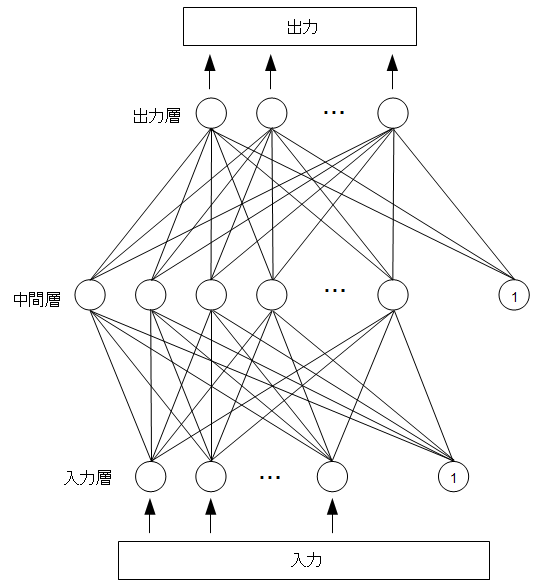
\includegraphics[width=0.45\hsize]{image201003/neuralnet01.png}
\end{center}
\end{figure}

それぞれの重みは実数で表され、パーセプトロンが機能するためにはこ
の重みが適切に設定されている必要があります。ある入力が与えられた
際、入力値に重みを掛け合わせ、それぞれの合計に次のようなシグモイ
ド関数を適用した数値を中間層の持つ値とします。

\begin{multicols}{2}

\begin{figure}[H]
\begin{center}
\caption{シグモイド関数の式}
\begin{equation*}
 \varsigma_1(x) = \frac{1}{1+e^{-x}}
\end{equation*}
\end{center}
\end{figure}

\begin{figure}[H]
\begin{center}
\caption{シグモイド関数のグラフ}
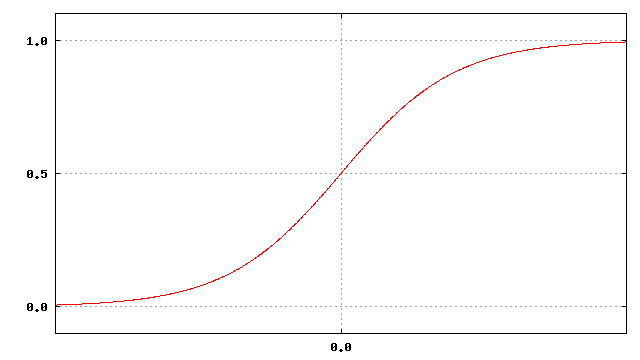
\includegraphics[width=1.0\hsize]{image201003/neuralnet03.png}
\end{center}
\end{figure}

\end{multicols}

各出力層も同様の計算がなされ、パーセプトロンの出力が行われます。

\subsubsection{バックプロパゲーション}

多層パーセプトロンで適切な出力を行うための学習方法として一般的な
ものにバックプロパゲーションがあります。バックプロパゲーションで
はまず入力に対する正しい出力(教師信号)を多数用意し、各重みをラン
ダムに設定します。用意された入力に対してランダムな重みからパーセ
プトロンの出力はでたらめな値となりますが、この出力と教師信号との
比較から出力層と中間層の間の重みを修正し、次いで中間層と入力層の
重みを修正することで適切な重みを探し出します。

\subsection{足し算と引き算を学習してみる}

作成したパーセプトロンとバックプロパゲーションが正常に動作するか
を確かめます。次のような入力を用意しました。

\begin{commandline}
# 学習用教師信号ペア
0.40,0.20	0.60,0.20
0.30,0.20	0.50,0.10
0.80,0.10	0.90,0.70
0.20,0.10	0.30,0.10
0.50,0.50	1.00,0.00
0.60,0.20	0.80,0.40
# 評価用入力値
*0.50,0.10
*0.50,0.40
*0.10,0.40
\end{commandline}

入力値と教師信号のペアはタブ区切りの左が入力、
右が入力に対する教師信号です。
ここでは足し算と引き算の教師信号を与えました。

\newpage

実行します。

\begin{commandline}
$ ./backprop.exe sample.txt 10000
       0 0.87640153
     100 0.26410368
     200 0.10289131
     300 0.03820243
     400 0.02475167

...(中略)...

    9600 0.00077714
    9700 0.00077174
    9800 0.00076646
    9900 0.00076128
0.4000, 0.2000  0.60, 0.18      0.60, 0.20
0.3000, 0.2000  0.50, 0.11      0.50, 0.10
0.8000, 0.1000  0.90, 0.70      0.90, 0.70
0.2000, 0.1000  0.30, 0.11      0.30, 0.10
0.5000, 0.5000  0.98, 0.02      1.00, 0.00
0.6000, 0.2000  0.80, 0.41      0.80, 0.40
0.5000, 0.1000  0.63, 0.35
0.5000, 0.4000  0.93, 0.06
0.1000, 0.4000  0.87, 0.00
Ratio=0.00075626
Count=10000
Sample=6
Input=2
Middle=4
Output=2
InputHidden0=-2.57936471,-2.20525001,-1.50656422,4.05055823,-0.66468037
InputHidden1=-1.29032439,8.71632107,-1.24344376,-0.85214732,-0.66468037
InputHidden2=2.04901840,-2.94096519,1.04866634,-1.98825291,0.29698485
HiddenOutput0=-2.91458436,-1.16992032
HiddenOutput1=5.84673832,-6.31188860
HiddenOutput2=-1.80018561,-0.42470539
HiddenOutput3=3.60356071,3.84028669
HiddenOutput4=1.40998866,-1.22885398
\end{commandline}

頼りないながらもそれなりの演算結果が出力されています。評価として
最後の数値は減算結果が負になるはずなのですが、シグモイド関数を通
すことで出力が0.0〜1.0となるため正常な結果が得られません。

\subsection{画像を分類するための入力値を考える}

画像判別の入力値として次の値を使用しました。

\begin{itemize}
\item 補正した画像のRGBの差
\item 微分した画像のRGBの差
\item 画像の複雑さ。
\item 使われている色の数
\item 平均彩度
\item FFT処理した画像の明るいピクセルを利用する
\item HSVに変換し、色素の平均を利用する
\item 色素の分散を利用する
\end{itemize}

この中から文章と絵の判別として画像のFFTを、カラー画像の判別とし
てHSVへの変換を解説します。

\subsubsection{モノクロ画像の処理・文字と絵を分類してみる}

縦書きの文章は横方向に一定の周波数を持っていると見なすことが出来
ます。これにより、文章の画像を微分しFFT処理を行った結果から振幅
を描画するとで、明るく光る点が現れることがわかりました。

\begin{figure}[H]
\begin{center}
\caption{イラストと文章を微分した画像のFFT結果}
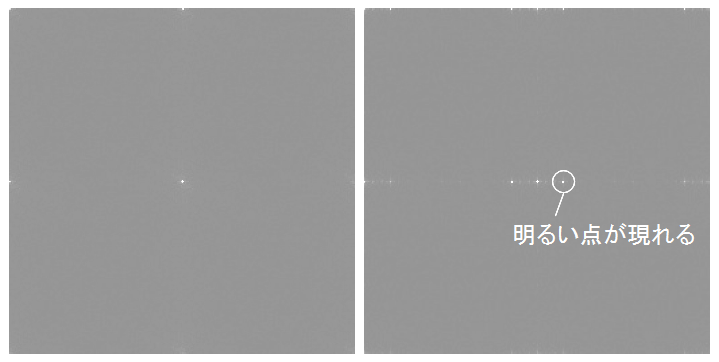
\includegraphics[width=0.9\hsize]{image201003/neuralnet04.png}
\end{center}
\end{figure}

この点の明るさを入力値とすることで、文章とイラストの判別が行える
と期待できます。

\subsubsection{カラー画像とそうでない画像を分類してみる}

カラー画像とモノクロ画像は画像のRGBをHSVに変換し、色相から判別を
行っています。

RGBのうちから最大のものをMAX、最小のものをMINとすると色相は次の
式となります。

\begin{figure}[H]
\begin{center}
\caption{色相の計算式}

\begin{align*}
 H = & 60 \frac{G-B}{MAX-MIN} + 0, & if MAX = R\\
     & 60 \frac{B-R}{MAX-MIN} + 120,   & if MAX = G\\
     & 60 \frac{R-G}{MAX-MIN} + 240,   & if MAX = B\\
\end{align*}
\end{center}
\end{figure}

モノクロ画像は色相を持たないため、RGBのうち青の成分を減らすこと
で黄色いフィルタをかけました。こうすることでモノクロ画像の色相の
平均は黄色となり、カラーとモノクロを判別するための入力値として期
待できます。

\subsection{学習の条件}

ニューラルネットの学習は次の条件で行いました。

\begin{itemize}
\item 入力層8個
\item 中間層24個
\item 出力層2個
\item サンプルとして使用した本23冊(漫画2冊/文庫20冊/技術書1冊)
\item ページ数6742ページ
\item 学習回数50万回
\end{itemize}

実際にこの条件で学習を行った際、
Core i7 950で7時間弱の学習時間となりました。

\subsection{判別の精度}

作成されたツールで実際に判別を行い、その精度を調べました。評価に
使用した本は学習に使われていないものを選びました。

\begin{description}
 \item[サンプル1. ライトノベル最新巻] \mbox{}\\
    240ページ中、人間の判別と食い違うページが2ページ。内訳はカラー
    12ページ、グレースケール15ページ、文章213ページ。そのうちイ
    ラストが文章と判別されたのが1ページ、文章がイラストと判別さ
    れたのが1ページ。
 \item[サンプル2. SF長編シリーズの上巻] \mbox{}\\
    568ページ中、人間の判別と食い違うページはなし。内訳はカラー5
    ページ、グレースケール3ページ、文章560ページ。
 \item[サンプル3. ローマ人のシリーズ1巻] \mbox{}\\
    216ページ中、人間の判別と食い違うページは5ページ。内訳はカラー
    6ページ、グレースケール9ページ、文章201ページ。そのうちカラー
    4ページの判別に失敗していますが、原因はカバーページがベージュ
    で文章として判別されました。地図やイラストと文章が混じったペー
    ジも学習通り文章として判別されています。
 \item[サンプル4. 50年前に発行された芥川賞受賞作] \mbox{}\\
    40年近く前に出版された本で、280ページ中、人間の判別と食い違
    うページが16ページ。内訳はカラー6ページ、文章274ページ。判別
    の失敗が多い理由は変色と推測され、カラーだけではなくイラスト
    とも多く間違って判別されました。
\end{description}

%-------------------------------------------------------------------------------
\dancersection{Wekaを使ってみる}{前田耕平}
%-------------------------------------------------------------------------------
\index{Weka}
\subsection{概要}

ニューラルネットワークをはじめとするデータマイニングを一般人が使うには、
本庄さんのネタのように理論を理解した上で自分でプログラムを作らないといけ
ないとすると、非常にハードルが高いと思います。学生のころに学んだり、研究
していたか、仕事として普段から扱っているような人でなければ、単語としては
耳にしたことがあっても、なんだかよう分からん、という人がほとんどではない
でしょうか。\footnote{Debian 勉強会の常連はむしろ知っている人の方が多い
のかもしれませんが、少なくとも私は単語を耳にしたことがあるレベルです。}
\index{でーたまいにんぐ@データマイニング}

そこで、バックグラウンドとしてニューラルネットワークだけでなく、データマ
イニングの基礎知識を持っていない私と同じような立場の人でも、Debian なら
気軽に試してみる環境を整えて、取り合えず使ってみることができるよ、という
趣旨で、Weka というツールを紹介します。

\subsection{Wekaとは}

Weka とは、``Waikato Environment for Knowledge Analysis''の略で、ニュー
ジーランドの国立ワイカト大学\footnote{\url{http://www.waikato.ac.nz/}}で
GPL のもとオープンソースで開発されているデータマイニングツールです。
\footnote{\url{http://www.cs.waikato.ac.nz/~ml/weka/index.html}} Java で
書かれています。

\subsection{インストール}

Debian ではパッケージが用意されています。

\begin{commandline}
$ sudo apt-get install weka
\end{commandline}

\subsection{Wekaの使い方}

コマンドラインで \texttt{weka} スクリプトを実行します。

\begin{commandline}
$ weka &
\end{commandline}

すると Weka のウィンドウが起動します。
そこから、``Applications'' の ``Explorer''を実行すると、
Weka Explorer が起動します。

\begin{figure}[H]
\begin{minipage}{0.4\hsize}
 \begin{center}
 \caption{Weka 起動メニュー}
 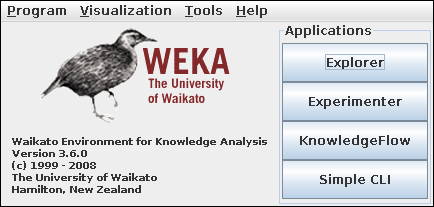
\includegraphics[width=1\hsize]{image201003/weka0.png}
 \end{center}
\end{minipage}
\begin{minipage}{0.5\hsize}
 \begin{center}
 \caption{Weka Explorer}
 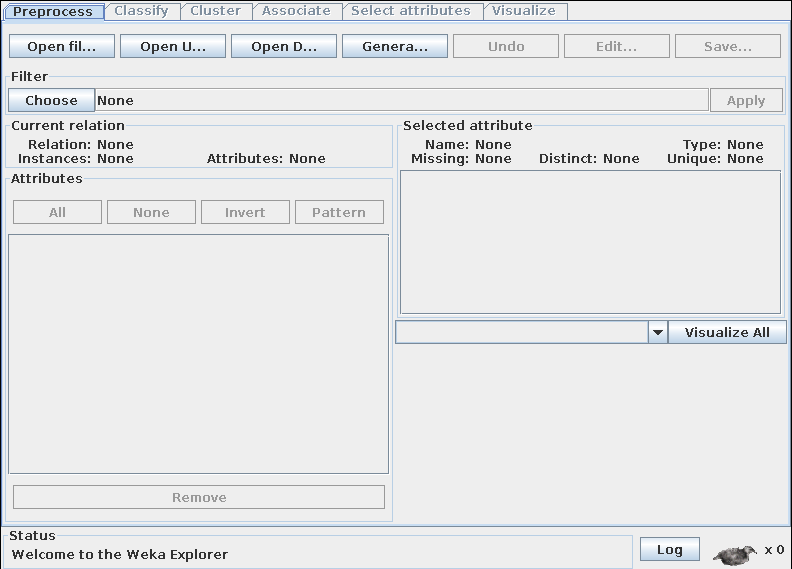
\includegraphics[width=1\hsize]{image201003/weka1.png}
 \end{center}
\end{minipage}
\end{figure}

\subsubsection{Weka で扱うデータフォーマット}

Weka では、ARFF(Attribute-Relation File Format)というフォーマットのテキ
ストファイルを入力データとして扱います。
\index{arff}

データフォーマットは次のようになります。

\begin{commandline}
@relation 名前
@attribute 属性名 属性の型
@attribute 属性名 属性の型
:
:
@data
データ,データ,…,データ
\end{commandline}

\begin{itemize}
\item @relation はデータ全体の名前を指定します。
\item @attribute はデータの属性を表し、1つ目の引数は属性名、2つめの引数
      は属性データの型を表します。
\item @attribute のデータ型には、numeric, real, integer, string, date型
      を使えます。
      \begin{itemize}
       \item numeric は real か integer を指定できます。
       \item real は実数を指定できます。
       \item integer は整数を指定できます。
       \item string は文字列を指定できます。
       \item date 型は日時で、デフォルトは''yyyy-MM-dd'T'HH:mm:ss''とい
	     う書式です。
      \end{itemize}
 \item @data データ領域の宣言です。
       \begin{itemize}
	\item その次の行から CSV 形式でデータを記述します。
	\item @attribute 行で上から設定した順に CSV の一行での左から右へ
	      の各データとなります。
       \end{itemize}
\end{itemize}

昨年の11月の勉強会で GNU R で扱った光熱費のデータと、気象庁が公開してい
る気温、降水量などの気象データ\footnote{\url{http://www.data.jma.go.jp/obd/stats/etrn/index.php}}を使ってみます。

まず、CSV で以下のように記述したとします。
\begin{commandline}
"年","月","降水量合計(mm)","平均日平均気温(℃)","平均日最高気温(℃)","平均日最低気
温(℃)","平均風速(m/s)","最大風速(m/s)","日照時間(h)","電気使用量(kWh)","電気使用
量(kWh)/日","料金(円)/日","合計料金","ガス使用量(m3)","ガス使用量(m3)/日","料金(
円)/日","合計料金"
2007,1,50,6,10.8,1.1,1,5,188.9,234,6.88235294117647,161.235294117647,5482,9,0.333333333333333,80.962962962963,2186
2007,2,44,7.3,12.6,1.9,1.3,6,198.1,198,7.07142857142857,168.071428571429,4706,9,0.321428571428571,87.7142857142857,2456
(snip)
\end{commandline}

これは、ARFF フォーマットでは以下のようになります。

\begin{commandline}
@relation 降水量・気温(府中市)と電気代、ガス代の関係について

@attribute 年 real
@attribute 月 real
@attribute 降水量合計(mm) real
@attribute 平均日平均気温(℃) real
@attribute 平均日最高気温(℃) real
@attribute 平均日最低気温(℃) real
@attribute 平均風速(m/s) real
@attribute 最大風速(m/s) real
@attribute 日照時間(h) real
@attribute 電気使用量(kWh) real
@attribute 電気使用量(kWh)/日 real
@attribute 料金(円)/日 real
@attribute 合計料金 real
@attribute ガス使用量(m3) real
@attribute ガス使用量(m3)/日 real
@attribute 料金(円)/日 real
@attribute 合計料金 real

@data
2007,1,50,6,10.8,1.1,1,5,188.9,234,6.88235294117647,161.235294117647,5482,9,0.333333333333333,80.962962962963,2186
2007,2,44,7.3,12.6,1.9,1.3,6,198.1,198,7.07142857142857,168.071428571429,4706,9,0.321428571428571,87.7142857142857,2456
(snip)
\end{commandline}

\subsubsection{ARFF をロードする}

先ほど用意した kohnetsu.arff をロードしてみましょう。Preprocess タブの
Open File ボタンを押します。ダイアログが表示されるので、kohnetsu.arff を
指定します。(\fgref{fig:wekaarffload})

ARFF ファイルを読み込むと\fgref{fig:wekaarffread}のようになります。UTF-8 エンコードであれば、
ご覧のとおり日本語も正常に読み込めます

\begin{figure}[H]
 \begin{minipage}{0.5\hsize}
  \begin{center}
   \caption{ARFF ファイルをロードする}
   \label{fig:wekaarffload}
   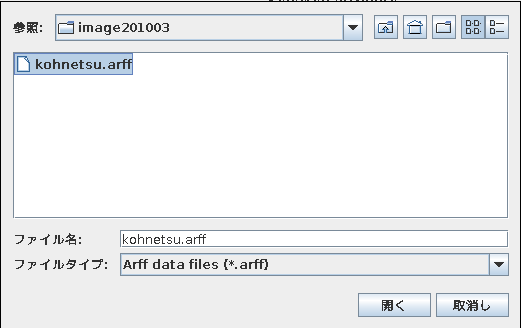
\includegraphics[width=0.9\hsize]{image201003/weka2.png}
  \end{center}
 \end{minipage}
 \begin{minipage}{0.5\hsize}
  \begin{center}
   \caption{ARFF からデータを読み込んだ結果}
   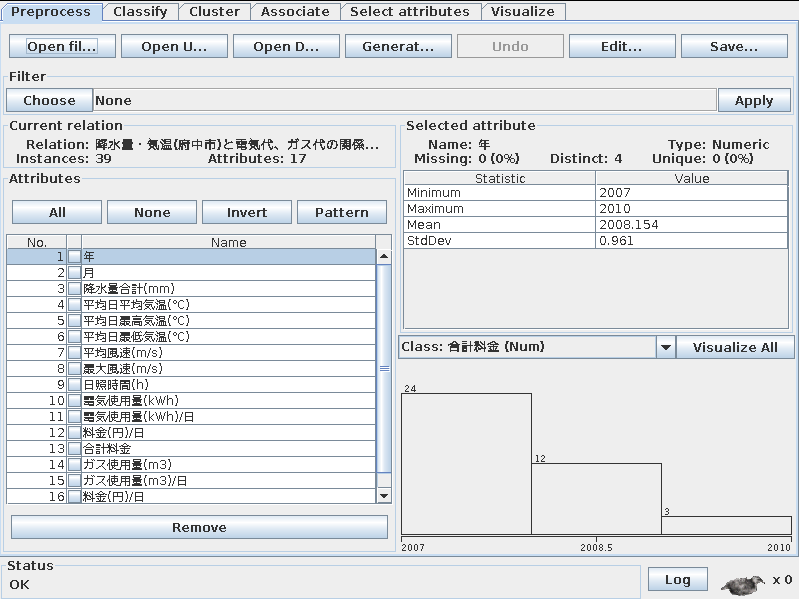
\includegraphics[width=0.9\hsize]{image201003/weka3.png}
   \label{fig:wekaarffread}
  \end{center}
 \end{minipage}
\end{figure}

\subsubsection{可視化してみる}

それでは読み込んだデータを可視化してみましょう。Visualize タブをクリック
すると\fgref{fig:wekavisualize}のようなマトリックスが表示されます。

適当に開いてみます。Y 軸に一日の平均気温の月平均(℃)と、 X 軸に一日あた
りの電気使用量(kWh)を取って見てみると\fgref{fig:wekavisualizedetail}のようになります。

\begin{figure}[H]
 \begin{minipage}{0.5\hsize}
\begin{center}
\caption{Visualize 画面}
\label{fig:wekavisualize}
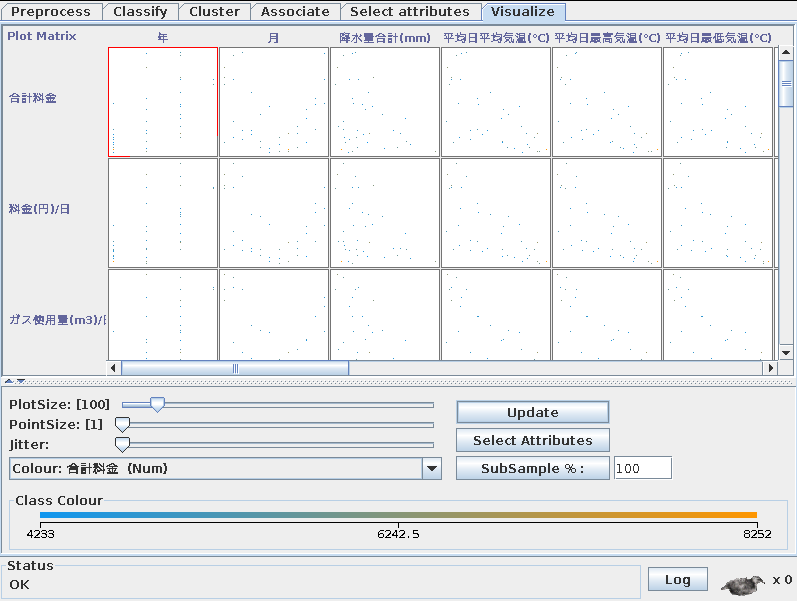
\includegraphics[width=1\hsize]{image201003/weka4.png}
\end{center}
\end{minipage}
\begin{minipage}{0.5\hsize}
 \begin{center}
 \caption{Visualize 詳細画面}
\label{fig:wekavisualizedetail}
 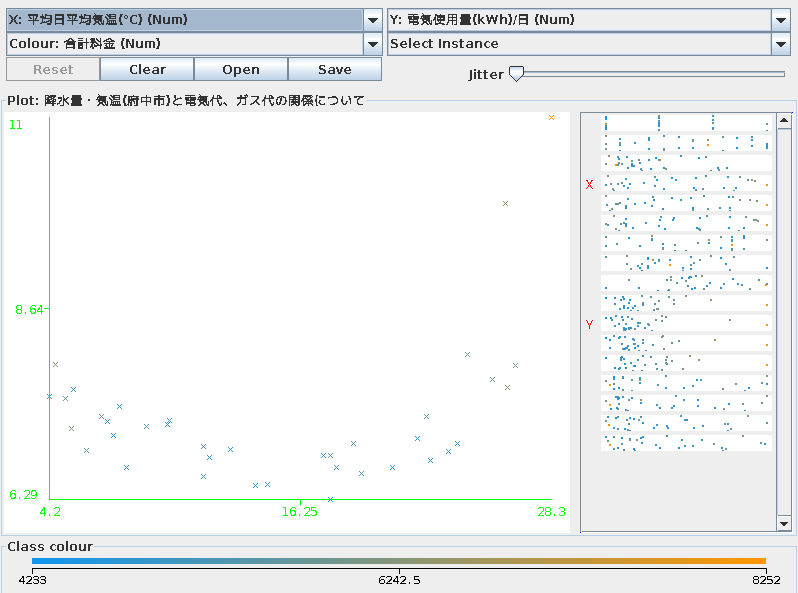
\includegraphics[width=1\hsize]{image201003/weka5.png}
 \end{center}
\end{minipage}
\end{figure}


\subsubsection{分類してみる}

次に分類してみます。Classify タブ → Choose ボタンを押し、表示されたツリー
からMultilayer Perceptron (ニューラルネットワークによる分類)を選択します。
次に、(Num)平均日平均気温(℃) を目的関数として選択します。
\index{neural network}

\begin{figure}[H]
\begin{center}
\caption{Classify 画面}
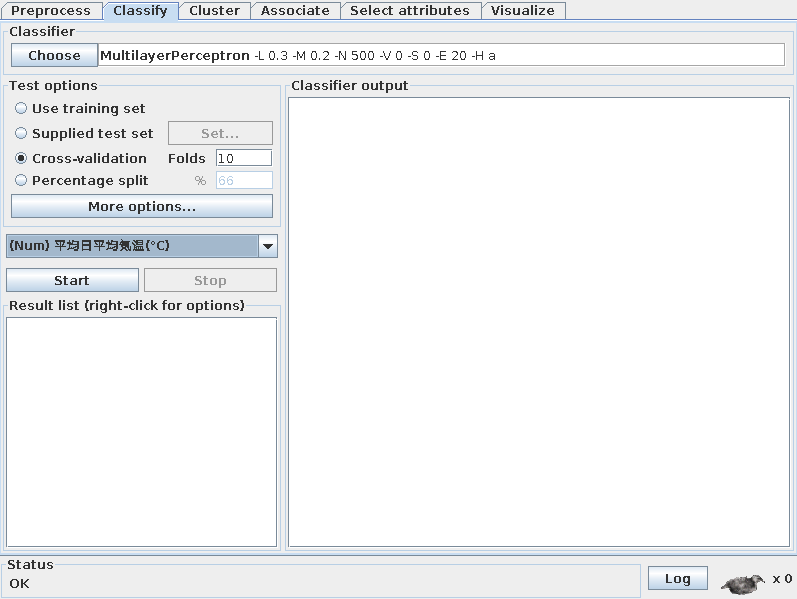
\includegraphics[width=0.6\hsize]{image201003/weka6.png}
\end{center}
\end{figure}

Start ボタンをクリックすると分類が実行され、結果が表示されます。

\begin{figure}[H]
\begin{center}
\caption{Classify 結果}
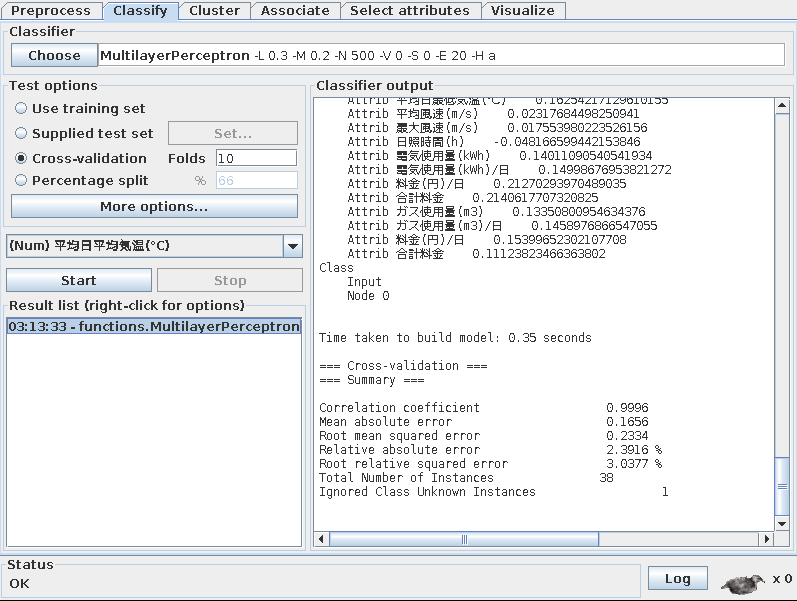
\includegraphics[width=0.6\hsize]{image201003/weka7.png}
\end{center}
\end{figure}

\subsubsection{予測してみる}

実は、kohnetsu.arff の最後の行(2010年3月のデータ)は、ほとんどの項目を'?'を入力
しています。

\begin{commandline}
2010,3,?,?,?,?,?,?,?,?,?,?,?,?,?,?,?
\end{commandline}

これはまだ今月のデータが出ていないからです。それでは、これらを予測してみ
ます。先ほどの Classify タブの画面で More options をクリックし、Output
predictions のチェックを入れ、OK を押します。

\begin{figure}[H]
\begin{center}
\caption{Classify の More Options ダイアログ}
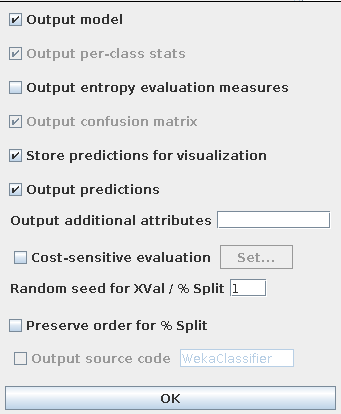
\includegraphics[width=0.4\hsize]{image201003/weka8.png}
\end{center}
\end{figure}

Start を実行すると、予測結果が表示されます。actual が実データで
predicted が予測結果です。今回見たいのは、3月の平均日平均気温です。
actual が ? になっている行の、predicted の値を見ると、15.436 となってい
ます。過去読み込ませたデータからニューラルネットワークでの分析して予測し
た結果、おそらく一日あたりの平均気温は 15.4 ℃ になるという予測です。来
月、気象庁の統計データが更新されたら確認してみましょう。

\begin{figure}[H]
\begin{center}
\caption{予測結果}
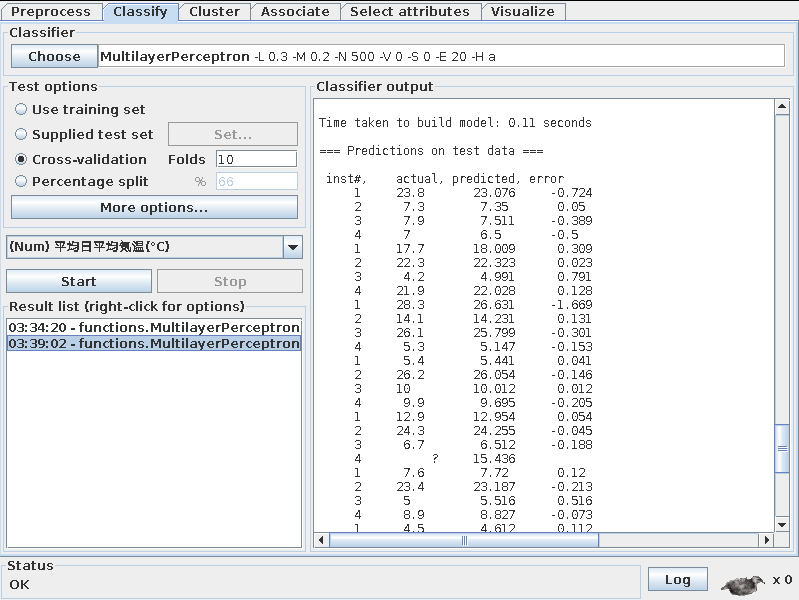
\includegraphics[width=0.6\hsize]{image201003/weka9.png}
\end{center}
\end{figure}

\subsection{まとめ}

なんとなく使えそうな気がしたでしょうか。私はこれで毎月のガス代、電気代、
さらには水道代の予測をして、給与日前日の予算計画に利用していこうと思いま
す。仕事でも、企画上の裏付けデータの分析、予測などにも使えそうですね。

\subsection{参考文献}
\begin{itemize}
 \item \url{http://www.ilibrary.jp/MOTtextBooks/text/weka.pdf}
 \item \url{http://web.sfc.keio.ac.jp/~soh/dm03/}
 \item \url{http://www1.doshisha.ac.jp/~mjin/R/23.pdf}
 \item \url{http://weka.wikispaces.com/ARFF}
\end{itemize}

%-------------------------------------------------------------------------------
\dancersection{man-db を深追いした}{日比野 啓}
%-------------------------------------------------------------------------------
\index{man-db}
\index{groff}

\subsection{日本語のmanが変}

こんな感じ\\
\includegraphics[width=75mm]{image201003/manls.eps}

日本語の文字の表示幅がアルファベットと同じだと判定されてしまっているので、
結果的に日本語で書かれた行の長さが倍ぐらいになってしまっています。

\subsection{解はgroffにあり}

\subsubsection{そもそもroffってどういうもの?}

簡単に言えば、タイプライターのようなものです。
いろいろなデバイスに対して印字を行なうことができるシステムになっていますが、
manでは文字端末に文字の幅と高さを考慮しながら印字をしていきます。

\subsubsection{roff文字幅の指定}

以前のバージョンのgroffでは日本語の文字の表示幅がアルファベットの倍であることを
unicodeのcode pointの範囲で設定してありました。
groffにはもともとcode pointの範囲で文字の幅を指定する機能が無いため、
その機能の追加と日本語文字の表示幅を倍にするパッチがあててありました。

更新されたバージョンにおいては日本語対応のパッチが当たらなくなってしまっていますが、
やはり同様の対処を行なう必要がありそうです。

% 最近はその日本語の文字の幅の指定が柔軟になったようですが、正しい設定がさ
% れていないようです。

%-------------------------------------------------------------------------------
\dancersection{Debian で libfftw を使ってみる}{上川純一}
%-------------------------------------------------------------------------------
\index{fftw}
\index{FFT}
\index{DFT}
\index{libfftw}
\index{libsndfile}

\subsection{はじめに}

DebianでFFTを取り扱うCのアプリケーションを書いてみたいと思うことはあり
ませんか?今日は音声データを分析してみましょう。

wav ファイルを入力として受け取り、FFTを実行してその結果を表示するアプリケー
ションを作成してみます。

\subsection{インストール}

libfftw3 をインストールします。
あと、音声ファイルをロードするために sndfile1 を利用します。

\begin{commandline}
$ apt-get install libfftw3-dev libsndfile1-dev
\end{commandline}
%$

\subsection{実験対象の準備:簡単なsine波を作成する}

まず、テスト用にFFTの結果が予想できるデータを作成してみます。
ここでは 440Hz のきれいなサイン波を作成しています。

\begin{equation*}
 data(x) = sin (\frac{2 \pi 440 x}{44100} ) 
\footnote{sin は radian}
\end{equation*}

\begin{commandline}
/*BINFMTC: -lsndfile -lm

  Create a sine wave at 44.1kHz for 1 second called sine.wav
 */
#include <stdlib.h>
#include <stdio.h>
#include <sndfile.h>
#include <math.h>

int create_sine(const char* filename, int size, double frequency)
{
  SF_INFO sfinfo = {
    .frames = size,
    .samplerate = 44100,
    .channels = 1,
    .format = SF_FORMAT_WAV | SF_FORMAT_PCM_16,
    .sections = 0,
    .seekable = 0
  };
  SNDFILE* s = sf_open(filename, SFM_WRITE, &sfinfo);
  double* data = malloc(sizeof(double) * size);
  int i;

  for (i=0; i < size; ++i)
    {
      data[i] = sin(frequency * 2.0 * M_PI * i / 44100.0);
    }

  sf_writef_double(s, data, size);
  sf_close(s);
  return 0;
}

int main()
{
  return create_sine("sine.wav", 44100, 440.0);
}
\end{commandline}

\subsection{実験対象の準備:複雑な入力値例の準備}

テスト用の入力値として、適当な wav ファイルを用意しましょう。

今回は手元で、aeolus というオルガンシミュレータを起動し、 
jack で接続させ、ecasound を jack 入力に
対して待機させ、qjackctl で接続させて収録しました。

それなりに長い時間録音したデータから 16-bit mono の PCM データ1秒分を切り
出して実験用データを作成しました。

\begin{commandline}
$ qjackctl &
$ aeolus &
$ vkeybd &
$ ecasound -i jack -o test.wav
ctrl-C で中断
$ sweep test.wav # 適当に編集
$ file ra-mono.wav  # 切り出した結果を確認
ra-mono.wav: RIFF (little-endian) data, WAVE audio, Microsoft PCM, 16 bit, mono 44100 Hz
\end{commandline}
%$

\subsection{FFTWを使って wav ファイルを処理してみる}

sndfile と fftw3 を使ってフーリエ変換して出力をダンプしてみましょう。サン
プルコードは sndfile を使い double の配列にwavファイルの中身を展開して、
その内容を fftw に渡して処理しています。double の値は各 1/44100 秒の瞬間
における空気の圧力を表しているようです。

\begin{commandline}
/*BINFMTC: -lsndfile -lfftw3 -lm
 */

#include <stdlib.h>
#include <stdio.h>
#include <sndfile.h>
#include <math.h>
#include <complex.h>
#include <fftw3.h>

/*
  process with FFTW
 */
void study_sound(double* data, int size)
{
  fftw_complex* spectrum;
  fftw_plan p;
  int i;

  spectrum = (fftw_complex*) fftw_malloc(sizeof(fftw_complex) * (size / 2 + 1));
  p = fftw_plan_dft_r2c_1d(size, data, spectrum, FFTW_ESTIMATE);

  /* process with FFTW */
  fftw_execute(p);

  /* dump output in CSV format */
  printf("i,abs,arg\n");
  for (i=0; i<(size/2+1); ++i) {
    printf("%i,%f,%f\n", i,
	   cabs(spectrum[i]),
	   carg(spectrum[i]) / 2.0 / M_PI * 360.0);
  }
  fftw_destroy_plan(p);
  fftw_free(spectrum);
}

/*
  Process wav file.

  @return 1 on failure, 0 on success.
*/
int process_wav_file(const char* filename, int size)
{
  SF_INFO sfinfo = {0, 0, 0, 0, 0, 0};
  SNDFILE* s = sf_open(filename, SFM_READ, &sfinfo);
  double* data = malloc(sizeof(double) * size);

  if (!s || !data)
    {
      fprintf(stderr,
	      "Something went wrong opening the file or allocating memory\n");
      return 1;
    }
  if (sfinfo.channels != 1)
    {
      fprintf(stderr,
	      "Please give me monaural audio data\n");
      return 1;
    }

  /* Read wav file into an array of double */
  sf_readf_double(s, data, size / sfinfo.channels);
  study_sound(data, size / sfinfo.channels);
  sf_close(s);
  return 0;
}

int main(int argc, char** argv)
{
  process_wav_file(argv[1], atoi(argv[2]));
  return 0;
}
\end{commandline}

実行してみます。

\begin{commandline}
$ ./sndfile-fftw.c sine.wav 44100 > sine.csv
$ ./sndfile-fftw.c ra-1sec.wav 44100 > ra.csv
\end{commandline}
%$

\subsection{出力を確認してみる}

CSVファイル形式でデータが出力されました。
簡単にグラフを作成するためのツールとしてここではRを使ってみます。

\begin{commandline}
$ R
> sine <- read.csv("sine.csv")
> ra <- read.csv("ra.csv")
> postscript("sine.eps", horizontal=FALSE, height=3, width=3)
> plot(sine$i, sine$abs, xlim=c(400,500), ylim=c(0,22000), type="l")
> dev.off()
> postscript("ra.eps", horizontal=FALSE, height=3, width=3)
> plot(ra$i, ra$abs, xlim=c(0,2000), ylim=c(0,100), type="l")
> dev.off()
\end{commandline}

\fgref{fig:wave-sine}の440Hz のサイン波を処理した結果を見てみると、440
Hz あたりにグラフの突起があるのが見て取れます。

しかし、実際にオルガン音を処理した結果の\fgref{fig:wave-ra}を見てみると、
グラフに突起が多数あって、結構複雑です。そのまま簡単に処理させてくれはし
なさそうです。

\begin{figure}[ht]
\begin{center}
 \begin{minipage}{0.4\hsize}
 \begin{center}
  \includegraphics{image201003/sine.eps}
 \end{center} 
 \label{fig:wave-sine}
 \caption{440Hz のサイン波}
 \end{minipage}
 \begin{minipage}{0.4\hsize}
 \begin{center}
  \includegraphics{image201003/ra.eps}
 \end{center} 
 \label{fig:wave-ra}
 \caption{ラをaeolusで適当に演奏した音}
 \end{minipage}
\end{center}
\end{figure}

%-------------------------------------------------------------------------------
\dancersection{dpkg ソース形式 ``3.0 (quilt)''}{吉野与志仁}
%-------------------------------------------------------------------------------
\subsection{はじめに}
普段Debianを使っている皆さんはご存知とは思いますが、近々デフォルトになる
予定でsqueezeのrelease goalであるDebianソースパッケー
ジのフォーマット``\verb|3.0 (quilt)|'' の復習をしたいと思います。
\subsection{``1.0''}
まずは``\verb|3.0 (quilt)|''の前に、いままで一般に使われてきたフォーマット(``\verb|1.0|'')を簡単にまとめます。

\verb|1.0|では、ソースパッケージは以下の3ファイルで構成されます。
\begin{itemize}
 \item \textit{packagename}\verb|-|\textit{upstreamversion}\verb|.orig.tar.gz|
 \item \textit{packagename}\verb|-|\textit{debianversion}\verb|.diff.gz|
 \item \textit{packagename}\verb|-|\textit{debianversion}\verb|.dsc|
\end{itemize}

なお、正確には\verb|1.0|は2種類あって、上の通常のパッケージのほかに``Debian
nativeな''パッケージがあります。Debian native パッケージは次の2ファイルで構成されます。
\begin{itemize}
 \item \textit{packagename}\verb|-|\textit{version}\verb|.tar.gz|
 \item \textit{packagename}\verb|-|\textit{version}\verb|.dsc|
\end{itemize}

ここで、\verb|*.orig.tar.gz|には、通常上流の元のソースツリーが含まれます。
\verb|*.diff.gz|には、ソースパッケージからパッケージなどをビルドするのに必要なスクリ
プトなどが入った \verb|debian/| ディレクトリや、上流のソースに対するパッケージ
メンテナの変更が含まれます。

\subsection{しかし}
と説明してきましたが、このファイル構成には
\begin{enumerate}
 \item アーカイブの圧縮形式に gzip しか使えない
 \item 複数のアーカイブで構成される上流のソースがそのまま扱えない
 \item メンテナが当てたソースへのパッチが全部つながってしまっている
 \item \verb|debian/| 以下にバイナリファイルが直接置けない
\end{enumerate}
などの問題点があります。

そこで、さまざまな方法が検討されました。

1は、これにより上流がbz2で配布していてもgzに圧縮し直さなければならなかっ
たりしていました。\verb|*.orig.tar.gz| の中身が上流のアーカイブの実体である、
といった方法なども(ちょっと無駄ですが...)使われてきました。この方法はビルド時にそのtarballを展開して作業
します。cdbsにはこの方法へのサポートもあります。

2は1と同様の方法で複数のtarballが入った\verb|*.orig.tar.gz|を用意したり
していました。

3は、当たっているパッチのそれぞれが
どんな意図で行われたのかがわからない、ということ、また、\verb|debian/|以下のファ
イルも上流ソースへのパッチも一緒くたになってしまっていること、が問題でした。そこで、まとまった意
味のある単位に分割されたパッチをまず用意しておき、それらを
\verb|debian/patches/| 下に配置
し、その細かいパッチをビル
ド時に当てる/外すフレームワーク
(patch system) が利用されています。これには dpatch や quilt などがありま
す。なお、この細かいパッチのそれぞれには、先頭にパッチの意図を説明する文
章を記述することが推奨されています(\url{http://dep.debian.net/deps/dep3/})。

4は、バイナリファイルのdiffを取ろうとしても普通のpatchではできないことが
原因なので、uuencodeなどでテキストに落としてpatchを取る、といった手法が
用いられてきました。

\subsection{そこで}
このような問題を解決するために新たなソースパッケージのフォーマットも検討
されました。それが``\verb|3.0 (quilt)|''フォーマット(と``\verb|3.0 (native)|''フォーマット)です。

\verb|3.0 (quilt)|は次の3つ以上のファイルで構成されます。
\begin{itemize}
 \item \textit{packagename}\verb|-|\textit{upstreamversion}\verb|.orig.tar.|\textit{ext}
 \item
      \textit{packagename}\verb|-|\textit{upstreamversion}\verb|.orig-|\textit{component}\verb|.tar.|\textit{ext}(任意)
 \item \textit{packagename}\verb|-|\textit{debianversion}\verb|.debian.tar.|\textit{ext}
 \item \textit{packagename}\verb|-|\textit{debianversion}\verb|.dsc|
\end{itemize}

なお、\verb|1.0|にあったDebian nativeパッケージに相当する\verb|3.0 (native)|は
次の2ファイルで構成されます。
\begin{itemize}
 \item \textit{packagename}\verb|-|\textit{version}\verb|.tar.|\textit{ext}
 \item \textit{packagename}\verb|-|\textit{version}\verb|.dsc|
\end{itemize}

ここで、まず、tarの拡張子部分\textit{ext}に gz のほか、bz2, lzma, xz が利用でき
るようになりました。これにより問題1が解決されました(\verb|3.0 (native)|に
おける主な変更点はこれです)。

また、\textit{component}の部分を適当に変えることにより複数のtarballをきち
んと扱えるようになりました。これが問題2を解決します。

次に、\verb|debian/|下のファイルはすべて \verb|*.debian.tar.gz| に入れることに
なりました。これですべてが混ざった状態はなくなりました。さら
に、\verb|debian/patches/| 下のパッチが、パッチシステム quilt と基本的に同じ方法
で \verb|dpkg-source(1)| によって``ソースパッケージの展開時に'' 自動的に当たる
ようになりました。これにより、ビルド時にパッチを当てるように \verb|debian/rules| ファイルを記述する必要はなく
なりましたし、\verb|debian/control|ファイルに\verb|Build-Depends: quilt|
などと書く必要もなくなりました。これらによって問題3は解決されました。

問題4については、\verb|debian/|下のファイルをdiffとして保持することはも
はやなくなったので解決し、\verb|*.debian.tar.|\textit{ext}に直にバイナリファイ
ルを配置できます。

\subsection{最近の動向}
この\verb|3.0 (quilt)|フォーマットは、Debianのアーカイブが巨大化していって
いるため、gzipよりlzma(lenny当時で、現在ならxz)を使って圧縮すればサイ
ズを抑えられるといった理由で、lenny以降でより推進されるようになりまし
た。Debianにあるソースパッケージすべてが\verb|3.0 (quilt)|化可能になった
ら(潰すべきminor/wishlistバグが
\url{http://bugs.debian.org/cgi-bin/pkgreport.cgi?users=hertzog@debian.org;tag=3.0-quilt-by-default}
にあります)、dpkg
はデフォルトで\verb|3.0 (quilt)|フォーマットでソースパッケージをビルドする
ように変更される、とのことです。というわけでこれから作るパッケージは3.0
化しましょう。

\subsection{例1:gzipパッケージ}
具体例として、まずgzipソースパッケージ(1.3.12-9)を\verb|3.0 (quilt)|化してみ
ました。このソースパッケージは直にpatchを当てた形式を取っていまし
た。\verb|dpkg-source(1)|による展開時のメッセージで分かります:
\begin{commandline}
$ apt-get source gzip
パッケージリストを読み込んでいます... 完了
依存関係ツリーを作成しています                
状態情報を読み取っています... 完了
479kB のソースアーカイブを取得する必要があります。
取得:1 http://ftp.jp.debian.org testing/main gzip 1.3.12-9 (dsc) [1,647B]
取得:2 http://ftp.jp.debian.org testing/main gzip 1.3.12-9 (tar) [462kB]
取得:3 http://ftp.jp.debian.org testing/main gzip 1.3.12-9 (diff) [15.7kB]
479kB を 1s で取得しました (250kB/s)
dpkg-source: info: extracting gzip in gzip-1.3.12
dpkg-source: info: unpacking gzip_1.3.12.orig.tar.gz
dpkg-source: info: applying gzip_1.3.12-9.diff.gz
dpkg-source: info: upstream files that have been modified: 
 gzip-1.3.12/.gbp.conf
 gzip-1.3.12/deflate.c
 gzip-1.3.12/gzip.1

(snip)
\end{commandline}
\subsubsection{バージョンの切り換え、ビルド}
現在のデフォルトは\verb|1.0|なので、\verb|3.0 (quilt)|と明示してからソー
スパッケージを作ります。
\begin{commandline}
$ cd gzip-1.3.12/
$ mkdir -p debian/source
$ echo '3.0 (quilt)' > debian/source/format
$ debuild -S -us -uc
 dpkg-buildpackage -rfakeroot -d -us -uc -S
dpkg-buildpackage: set CFLAGS to default value: -g -O2

(snip)

 dpkg-source -b gzip-1.3.12
dpkg-source: info: using source format `3.0 (quilt)'
dpkg-source: info: building gzip using existing ./gzip_1.3.12.orig.tar.gz
dpkg-source: info: local changes stored in gzip-1.3.12/debian/patches/debian-changes-1.3.12-9, the modified files are:
 gzip-1.3.12/.gbp.conf
 gzip-1.3.12/deflate.c

(snip)

dpkg-source: info: building gzip in gzip_1.3.12-9.debian.tar.gz
dpkg-source: info: building gzip in gzip_1.3.12-9.dsc
 dpkg-genchanges -S >../gzip_1.3.12-9_source.changes

(snip)
\end{commandline}
と、とりあえず昔のdiff.gz(の上流ソースへのパッチ部分)に相当する1つのパッ
チを自動で出力してくれます。この大きなパッチそのままではこのフォーマット
にした意味がほとんどないので分けましょう。また、パッチの説明文テンプレー
トも\verb|debian/changelog|を基にして付けてくれるので、修正して正しい説明にしましょう。(今回は
共に省略)

バイナリパッケージをビルドしてみます。
\begin{commandline}
$ debuild -b -us -uc
 dpkg-buildpackage -rfakeroot -D -us -uc -b
dpkg-buildpackage: set CFLAGS to default value: -g -O2
dpkg-buildpackage: set CPPFLAGS to default value: 
dpkg-buildpackage: set LDFLAGS to default value: 
dpkg-buildpackage: set FFLAGS to default value: -g -O2
dpkg-buildpackage: set CXXFLAGS to default value: -g -O2
dpkg-buildpackage: source package gzip
dpkg-buildpackage: source version 1.3.12-9
dpkg-buildpackage: source changed by Bdale Garbee <bdale@gag.com>
dpkg-buildpackage: host architecture amd64
dpkg-checkbuilddeps: Unmet build dependencies: mingw32
dpkg-buildpackage: warning: Build dependencies/conflicts unsatisfied; aborting.
dpkg-buildpackage: warning: (Use -d flag to override.)
debuild: fatal error at line 1330:
dpkg-buildpackage -rfakeroot -D -us -uc -b failed
\end{commandline}
\verb|Build-Depends|を満たして、ビルドします。
\begin{commandline}
$ mk-build-deps 
dh_testdir

(snip) 

dpkg-deb: `../gzip-build-deps_1.0_all.deb' にパッケージ `gzip-build-deps' を構築しています。

The package has been created.
Attention, the package has been created in the current directory,
not in ".." as indicated by the message above!
$ sudo dpkg -i gzip-build-deps_1.0_all.deb
未選択パッケージ gzip-build-deps を選択しています。
(データベースを読み込んでいます ... 現在 203017 個のファイルとディレクトリがインストールされています。)
(gzip-build-deps_1.0_all.deb から) gzip-build-deps を展開しています...
dpkg: 依存関係の問題により gzip-build-deps の設定ができません:
 gzip-build-deps は以下に依存 (depends) します: mingw32 ...しかし:
  パッケージ mingw32 はまだインストールされていません。
dpkg: gzip-build-deps の処理中にエラーが発生しました (--install):
 依存関係の問題 - 設定を見送ります
以下のパッケージの処理中にエラーが発生しました:
 gzip-build-deps
$ sudo aptitude install gzip-build-deps
パッケージリストを読み込んでいます... 完了

(snip)

タスクの記述を読み込んでいます... 完了  

現在の状態: 依存関係破損が 0 個 [-1]。
$ debuild -b -us -uc
 dpkg-buildpackage -rfakeroot -D -us -uc -b
dpkg-buildpackage: set CFLAGS to default value: -g -O2

(snip)

dpkg-deb: `../gzip_1.3.12-9_amd64.deb' にパッケージ `gzip' を構築しています。
 dpkg-genchanges -b >../gzip_1.3.12-9_amd64.changes
dpkg-genchanges: binary-only upload - not including any source code
dpkg-buildpackage: binary only upload (no source included)
Now running lintian...
W: gzip: missing-dependency-on-install-info
Finished running lintian.
\end{commandline}
\subsection{例2:bash-completionパッケージ}
次に、パッチシステムとしてquiltを使っていたbash-completionパッケージを
\verb|3.0 (quilt)|化してみました。

\subsubsection{まずビルド}
パッチシステムでは、ビルド前はパッチは当たっていないので、自動でツリーに
パッチが当てられてソースパッケージがビルドされます。
\begin{commandline}
$ apt-get source bash-completion
パッケージリストを読み込んでいます... 完了

(snip)

$ cd bash-completion-1.1/
$ mkdir -p debian/source
$ echo '3.0 (quilt)' > debian/source/format
$ debuild -S -us -uc
 dpkg-buildpackage -rfakeroot -d -us -uc -S
dpkg-buildpackage: set CFLAGS to default value: -g -O2

(snip)

 fakeroot debian/rules clean
dh --with quilt clean
   dh_testdir
   dh_auto_clean
   dh_quilt_unpatch
適用されているパッチはありません
   dh_clean
 dpkg-source -b bash-completion-1.1
dpkg-source: info: using source format `3.0 (quilt)'
dpkg-source: warning: patches have not been applied, applying them now (use --no-preparation to override)
dpkg-source: info: applying 01-fix_550943.patch
dpkg-source: info: applying 02-fix_552109.patch
dpkg-source: info: applying 03-fix_552631.patch
dpkg-source: info: building bash-completion using existing ./bash-completion_1.1.orig.tar.gz
dpkg-source: info: building bash-completion in bash-completion_1.1-3.debian.tar.gz
dpkg-source: info: building bash-completion in bash-completion_1.1-3.dsc
 dpkg-genchanges -S >../bash-completion_1.1-3_source.changes

(snip)
\end{commandline}
今回は問題ありませんでしたが、\verb|3.0 (quilt)|はquiltとは微妙に異なり、す
べて \verb|patch -p1| として扱われるのでpathを適当に調整する必要があるか
もしれません。
\subsubsection{quilt周りの変更}
パッチは展開時に当たるので、\verb|debian/rules|内でパッチを当てている部
分はもう要りません。このソースパッケージは\verb|dh(1)|を使用していたので簡単でした。
\begin{commandline}
--- debian/rules	2010-03-18 10:50:30.000000000 +0900
+++ debian/rules.new	2010-03-18 10:54:53.000000000 +0900
@@ -21,11 +21,11 @@
 
 build: build-stamp
 build-stamp:
-	dh --with quilt build
+	dh build
 	touch $@
 
 clean:
-	dh --with quilt $@
+	dh $@
 
 install: install-stamp
 install-stamp: build
\end{commandline}
quiltには通常は\verb|Build-Depends|しません。
\begin{commandline}
--- debian/control	2010-03-18 10:50:30.000000000 +0900
+++ debian/control.new	2010-03-18 10:57:00.000000000 +0900
@@ -3,7 +3,7 @@
 Priority: standard
 Maintainer: Bash Completion Maintainers <bash-completion-devel@lists.alioth.debian.org>
 Uploaders: David Paleino <dapal@debian.org>
-Build-Depends: debhelper (>= 7.0.50), quilt (>= 0.46-7~)
+Build-Depends: debhelper (>= 7.0.50)
 Build-Depends-Indep: perl
 Standards-Version: 3.8.3
 Vcs-Git: git://git.debian.org/git/bash-completion/debian.git
\end{commandline}
\subsubsection{もう一回}
今度は初めから\verb|3.0 (quilt)|です。
\begin{commandline}
$ debuild -S -us -uc
 dpkg-buildpackage -rfakeroot -d -us -uc -S

(snip)

 fakeroot debian/rules clean
dh clean
   dh_testdir
   dh_auto_clean
   dh_clean
 dpkg-source -b bash-completion-1.1
dpkg-source: info: using source format `3.0 (quilt)'
dpkg-source: info: building bash-completion using existing ./bash-completion_1.1.orig.tar.gz
dpkg-source: info: building bash-completion in bash-completion_1.1-3.debian.tar.gz
dpkg-source: info: building bash-completion in bash-completion_1.1-3.dsc
 dpkg-genchanges -S >../bash-completion_1.1-3_source.changes
dpkg-genchanges: not including original source code in upload
dpkg-buildpackage: binary and diff upload (original source NOT included)
Now running lintian...
Finished running lintian.
\end{commandline}
バイナリパッケージをビルドします。
\begin{commandline}
$ debuild -b -us -uc
 dpkg-buildpackage -rfakeroot -D -us -uc -b
dpkg-buildpackage: set CFLAGS to default value: -g -O2

(snip)

dpkg-deb: `../bash-completion_1.1-3_all.deb' にパッケージ `bash-completion' を構築しています。
 dpkg-genchanges -b >../bash-completion_1.1-3_amd64.changes
dpkg-genchanges: binary-only upload - not including any source code
dpkg-buildpackage: binary only upload (no source included)
Now running lintian...
Finished running lintian.
\end{commandline}
\subsection{例3:ptex-binパッケージ}
次に、実際には複数のソースアーカイブを使用しているptex-binソー
スパッケージ(3.1.11+0.04b-0.1)を\verb|3.0 (quilt)|化してみました。

ptex-binソースパッケージは、実際には \verb|ptex-src-*.tar.gz| と \verb|jmpost-*.tar.gz| の2
つの上流tarballから構成されます。さらに\verb|Build-Depends: ptex-buildsupport|となっていますが、このptex-buildsupportパッケージは
\verb|tetex-src-*-stripped.tar.gz|のみが含まれる、ほぼビルド専用のパッケー
ジです。すなわち、3つの上流tarballが使われています。その上、このソースパッ
ケージには \verb|debian/patches/|ディレクトリがありますが、quiltやdpatch
といった近代的なものではなくビルド時にpatchを\verb|debian/rules|内で直接呼ぶ構成になっていま
した。
\subsubsection{ソースの用意、名前の変更}
\begin{commandline}
 $ apt-get source ptex-bin
 $ apt-get source ptex-buildsupport
\end{commandline}
適当に名前を変えます。ここでは
\begin{commandline}
$ mv ptex-bin-3.1.11+0.04b/ptex-src-3.1.11.tar.gz ptex-bin_3.1.11+0.04b+3.0.orig.tar.gz
$ mv ptex-bin-3.1.11+0.04b/jmpost-0.04b.tar.gz ptex-bin_3.1.11+0.04b+3.0.orig-jmpost.tar.gz
$ mv ptex-buildsupport-3.0/tetex-src-3.0-stripped.tar.gz ptex-bin_3.1.11+0.04b+3.0.orig-tetex-stripped.tar.gz
\end{commandline}
としました。\verb|3.0 (quilt)|では、\verb|*.orig.tar.|\textit{ext}がまずメインで展開され、そのソースツ
リーに\textit{component}ディレクトリが掘られてその下に各
\verb|*.orig-|\textit{component}\verb|.tar.|\textit{ext}が展開されます。ま
た、\textit{component}には英数字とハイフンのみが使えます。
\subsubsection{とりあえずビルド}
\begin{commandline}
$ mkdir ptex-bin-3.1.11+0.04b+3.0
$ cd ptex-bin-3.1.11+0.04b+3.0/
$ cp -a ../ptex-bin-3.1.11+0.04b/debian .
$ mkdir -p debian/source
$ echo '3.0 (quilt)' > debian/source/format
$ dch -v 3.1.11+0.04b+3.0-0.1
(適当にchangelog追加)
$ debuild -S -us -uc
 dpkg-buildpackage -rfakeroot -d -us -uc -S
dpkg-buildpackage: set CFLAGS to default value: -g -O2
dpkg-buildpackage: set CPPFLAGS to default value: 
dpkg-buildpackage: set LDFLAGS to default value: 
dpkg-buildpackage: set FFLAGS to default value: -g -O2
dpkg-buildpackage: set CXXFLAGS to default value: -g -O2
dpkg-buildpackage: source package ptex-bin
dpkg-buildpackage: source version 3.1.11+0.04b+3.0-0.1
dpkg-buildpackage: source changed by YOSHINO Yoshihito <yy.y.ja.jp@gmail.com>
 fakeroot debian/rules clean
dh_testdir
dh_testroot
rm -f build-stamp configure-stamp
# Add here commands to clean up after the build process.
# Remove teTeX source directory.
rm -rf tetex-src-3.0
dh_clean
dh_clean: Compatibility levels before 5 are deprecated.
 dpkg-source -b ptex-bin-3.1.11+0.04b+3.0
dpkg-source: info: using source format `3.0 (quilt)'
dpkg-source: info: building ptex-bin using existing ./ptex-bin_3.1.11+0.04b+3.0.
orig-jmpost.tar.gz ./ptex-bin_3.1.11+0.04b+3.0.orig-tetex-stripped.tar.gz ./ptex
-bin_3.1.11+0.04b+3.0.orig.tar.gz
dpkg-source: warning: ignoring deletion of file kanji.defines
dpkg-source: warning: ignoring deletion of file pconvert
dpkg-source: warning: ignoring deletion of file tftopl.ch

(snip)

dpkg-source: info: building ptex-bin in ptex-bin_3.1.11+0.04b+3.0-0.1.debian.tar
.gz
dpkg-source: info: building ptex-bin in ptex-bin_3.1.11+0.04b+3.0-0.1.dsc
 dpkg-genchanges -S >../ptex-bin_3.1.11+0.04b+3.0-0.1_source.changes
\end{commandline}
とりあえず空のソースツリーで作ったのでソースがないというwarningはスルー
します。
\begin{commandline}
$ cd ..
$ dpkg-source -x ptex-bin_3.1.11+0.04b+3.0-0.1.dsc
dpkg-source: warning: extracting unsigned source package (ptex-bin_3.1.11+0.04b+3.0-0.1.dsc)
dpkg-source: info: extracting ptex-bin in ptex-bin-3.1.11+0.04b+3.0
dpkg-source: info: unpacking ptex-bin_3.1.11+0.04b+3.0.orig.tar.gz
dpkg-source: info: unpacking ptex-bin_3.1.11+0.04b+3.0.orig-jmpost.tar.gz
dpkg-source: info: unpacking ptex-bin_3.1.11+0.04b+3.0.orig-tetex-stripped.tar.gz
dpkg-source: info: unpacking ptex-bin_3.1.11+0.04b+3.0-0.1.debian.tar.gz
$ cd -
$ ls -F
COPYRIGHT      README.txt   jbibtex.ch       mkconf        ptexextra.h
COPYRIGHT.jis  configure*   jbibtex.defines  pconvert*     ptexhelp.h
Changes.txt    debian/      jmpost/          pdvitype.ch   tetex-stripped/
Files          jbibd.sed    kanji.c          pltotf.ch     tftopl.ch
INSTALL.txt    jbibextra.c  kanji.defines    ptex-base.ch  usage.c
Makefile.in    jbibextra.h  kanji.h.in       ptexextra.c   version.c
\end{commandline}
メインのソースのトップディレクトリでそのままビルドできるようなものはいい
ですが、\verb|ptex-src-*.tar.gz|はそうではないので微妙ですね... ともか
く、今回はビルド用ディレクトリを掘ってビルドできるように\verb|debian/rules|の変
更が必要でした。
\subsubsection{quilt化}
普段パッチシステムquiltを使っていればほとんど変更の必要はありませんが、
このパッケージはパッチは分かれているものの自力で色々やっているので
まずquilt化が必要でした。

全パッチを\verb|-p1|化した上で、\verb|debian/rules|に書かれている通りの
順番でパッチを\verb|quilt import && quilt push|
しました。quiltでは同じパッチ名はダメのようですね。
\begin{commandline}
$ cd debian/
$ mv patches patches.old
$ sed -i 's@^\(---\|+++\) @&ptex-bin-3.1.11+0.04b+3.0/tetex-stripped/@' patches.old/teTeX/*.patch
$ sed -i 's@^\(---\|+++\) @&ptex-bin-3.1.11+0.04b+3.0/@' patches.old/*.patch
$ sed -i 's@^\(---\|+++\) @&ptex-bin-3.1.11+0.04b+3.0/jmpost/@' patches.old/jmpost/*.patch
$ mv patches.old/Makefile.in.patch patches.old/pTeX_Makefile.in.patch
$ mv patches.old/jmpost/Makefile.in.patch patches.old/jmpost/jmpost_Makefile.in.patch
$ quilt import patches.old/teTeX/*.patch patches.old/*.patch patches.old/jmpost/*.patch
パッチ patches.old/teTeX/Makefile.in.patch を取り込んでいます (Makefile.in.patch として保存されます)
パッチ patches.old/teTeX/common.mk.patch を取り込んでいます (common.mk.patch として保存されます)
パッチ patches.old/teTeX/config.h.patch を取り込んでいます (config.h.patch として保存されます)
パッチ patches.old/teTeX/depend.mk.patch を取り込んでいます (depend.mk.patch として保存されます)
パッチ patches.old/teTeX/splitup.c.patch を取り込んでいます (splitup.c.patch として保存されます)
パッチ patches.old/teTeX/web2c.depend.mk.patch を取り込んでいます (web2c.depend.mk.patch として保存されます)
パッチ patches.old/pTeX_Makefile.in.patch を取り込んでいます (pTeX_Makefile.in.patch として保存されます)
パッチ patches.old/jmpost/jmpost_Makefile.in.patch を取り込んでいます (jmpost_Makefile.in.patch として保存されます)
$ cd ..
$ env QUILT_PATCHES=debian/patches quilt push -a
パッチ Makefile.in.patch を適用しています
patching file tetex-stripped/texk/web2c/web2c/Makefile.in

パッチ common.mk.patch を適用しています
patching file tetex-stripped/texk/make/common.mk

パッチ config.h.patch を適用しています
patching file tetex-stripped/texk/web2c/config.h

パッチ depend.mk.patch を適用しています
patching file tetex-stripped/texk/web2c/lib/depend.mk

パッチ splitup.c.patch を適用しています
patching file tetex-stripped/texk/web2c/web2c/splitup.c

パッチ web2c.depend.mk.patch を適用しています
patching file tetex-stripped/texk/web2c/web2c/depend.mk

パッチ pTeX_Makefile.in.patch を適用しています
patching file Makefile.in

パッチ jmpost_Makefile.in.patch を適用しています
patching file jmpost/Makefile.in

現在位置はパッチ jmpost_Makefile.in.patch です
$ rm -r debian/patches.old/
\end{commandline}
\subsubsection{debian/rules, debian/controlの変更}
tarballをもう展開する必要はありません。ビルド用ディレクトリにコピーするこ
とにします。パッチを当てる必要もないのでその辺も削ります。
\begin{commandline}
--- debian/rules	2010-03-18 12:01:15.000000000 +0900
+++ debian/rules.new	2010-03-18 13:19:09.000000000 +0900
@@ -6,29 +6,14 @@
 # Uncomment this to turn on verbose mode.
 #export DH_VERBOSE=1
 
-####################
-# Things you should change when new upstream version is available.
-
-# Minimal teTeX source tarball.
-# You should install ptex-buildsupport package beforehand.
-TETEX_SRC_TARBALL=/usr/src/tetex-src-3.0-stripped.tar.gz
-
 # teTeX source directory.
-TETEX_SRC_DIR=tetex-src-3.0
-
-# pTeX source tarball.
-PTEX_SRC_TARBALL=ptex-src-3.1.11.tar.gz
+TETEX_SRC_DIR=tetex-src
 
 # pTeX source directory.
-PTEX_SRC_DIR=ptex-src-3.1.11
-
-# Japanized MetaPost tarball.
-JMPOST_SRC_TARBALL=jmpost-0.04b.tar.gz
+PTEX_SRC_DIR=ptex-src
 
 # Japanized MetaPost source directory.
-JMPOST_SRC_DIR=jmpost-0.04b
-
-####################
+JMPOST_SRC_DIR=jmpost-src
 
 DEB_HOST_GNU_TYPE	:= $(shell dpkg-architecture -qDEB_HOST_GNU_TYPE)
 
@@ -42,31 +27,14 @@
 configure: configure-stamp
 configure-stamp:
 	dh_testdir
-	# Unpack tarballs.
-	tar xfz $(TETEX_SRC_TARBALL)
+	cp -al tetex-stripped $(TETEX_SRC_DIR)
 	mkdir $(TETEX_SRC_DIR)/texk/kpathsea_tetex
 	mv $(TETEX_SRC_DIR)/texk/kpathsea/c-proto.h $(TETEX_SRC_DIR)/texk/kpathsea_tetex/
 	rm -rf $(TETEX_SRC_DIR)/texk/kpathsea
 	ln -s /usr/include/kpathsea $(TETEX_SRC_DIR)/texk/kpathsea
-	tar xfz $(PTEX_SRC_TARBALL) -C $(TETEX_SRC_DIR)/texk/web2c
-	tar xfz $(JMPOST_SRC_TARBALL) -C $(TETEX_SRC_DIR)/texk/web2c/$(PTEX_SRC_DIR)
-
-	# Apply patches to teTeX source
-	for f in debian/patches/teTeX/*.patch; do \
-		patch -p0 -d $(TETEX_SRC_DIR) < $$f; \
-	done
-
-	# Apply patches to pTeX source (should be named as *.patch)
-	# Put patches in debian/patches.
-	(for f in debian/patches/*.patch ; do \
-	  patch -p0 -d $(TETEX_SRC_DIR)/texk/web2c/$(PTEX_SRC_DIR) < $$f ; \
-	done)
-
-	# Apply patches to Japanized MetaPost source (should be named as *.patch)
-	# Put patches in debian/patches/jmpost.
-	(for f in debian/patches/jmpost/*.patch ; do \
-	  patch -p0 -d $(TETEX_SRC_DIR)/texk/web2c/$(PTEX_SRC_DIR)/$(JMPOST_SRC_DIR) < $$f ; \
-	done)
+	mkdir $(TETEX_SRC_DIR)/texk/web2c/$(PTEX_SRC_DIR)
+	for f in `find . -maxdepth 1 -type f`; do cp -al $$f $(TETEX_SRC_DIR)/texk/web2c/$(PTEX_SRC_DIR); done
+	cp -al jmpost $(TETEX_SRC_DIR)/texk/web2c/$(PTEX_SRC_DIR)/$(JMPOST_SRC_DIR)
 
 	# Copy texmf.cnf from your system.
 	cp /usr/share/texmf/web2c/texmf.cnf \
\end{commandline}
ptex-buildsupportは不要になりました。
\begin{commandline}
--- debian/control	2010-03-18 12:01:15.000000000 +0900
+++ debian/control.new	2010-03-18 13:23:09.000000000 +0900
@@ -2,7 +2,7 @@
 Section: tex
 Priority: optional
 Maintainer: Masayuki Hatta (mhatta) <mhatta@debian.org>
-Build-Depends: debhelper (>> 4.0.0), texlive-binaries,
 texlive-extra-utils, texlive-metapost, flex, bison, libkpathsea-dev, \
ptex-base (>= 2.4), ptex-buildsupport (>= 3.0), libtool
+Build-Depends: debhelper (>> 4.0.0), texlive-binaries,
 texlive-extra-utils, texlive-metapost, flex, bison, libkpathsea-dev, \
ptex-base (>= 2.4), libtool
 Standards-Version: 3.7.3
 
 Package: ptex-bin
\end{commandline}
\subsubsection{ビルド}
\begin{commandline}
$ debuild -S -us -uc
 dpkg-buildpackage -rfakeroot -d -us -uc -S
dpkg-buildpackage: set CFLAGS to default value: -g -O2

(snip)
\end{commandline}
試しに\verb|dpkg-source -x|してみます。
\begin{commandline}
$ dpkg-source -x ptex-bin_3.1.11+0.04b+3.0-0.1.dsc
dpkg-source: warning: extracting unsigned source package (ptex-bin_3.1.11+0.04b+3.0-0.1.dsc)
dpkg-source: info: extracting ptex-bin in ptex-bin-3.1.11+0.04b+3.0
dpkg-source: info: unpacking ptex-bin_3.1.11+0.04b+3.0.orig.tar.gz
dpkg-source: info: unpacking ptex-bin_3.1.11+0.04b+3.0.orig-jmpost.tar.gz
dpkg-source: info: unpacking ptex-bin_3.1.11+0.04b+3.0.orig-tetex-stripped.tar.gz
dpkg-source: info: unpacking ptex-bin_3.1.11+0.04b+3.0-0.1.debian.tar.gz
dpkg-source: info: applying Makefile.in.patch
dpkg-source: info: applying common.mk.patch
dpkg-source: info: applying config.h.patch
dpkg-source: info: applying depend.mk.patch
dpkg-source: info: applying splitup.c.patch
dpkg-source: info: applying web2c.depend.mk.patch
dpkg-source: info: applying pTeX_Makefile.in.patch
dpkg-source: info: applying jmpost_Makefile.in.patch
\end{commandline}
無事当たりました。
バイナリパッケージをビルドします。
\begin{commandline}
$ debuild -b -us -uc
 dpkg-buildpackage -rfakeroot -D -us -uc -b
dpkg-buildpackage: set CFLAGS to default value: -g -O2

(snip)

dpkg-buildpackage: warning: Build dependencies/conflicts unsatisfied; aborting.
dpkg-buildpackage: warning: (Use -d flag to override.)
debuild: fatal error at line 1330:
dpkg-buildpackage -rfakeroot -D -us -uc -b failed
$ mk-build-deps

(snip)

$ sudo dpkg -i ptex-bin-build-deps_1.0_all.deb 

(snip)

$ sudo aptitude install ptex-bin-build-deps

(snip)

$ debuild -b -us -uc
 dpkg-buildpackage -rfakeroot -D -us -uc -b
dpkg-buildpackage: set CFLAGS to default value: -g -O2

(snip)

dh_builddeb
dh_builddeb: Compatibility levels before 5 are deprecated.
dpkg-deb: `../ptex-bin_3.1.11+0.04b+3.0-0.1_amd64.deb' にパッケージ `ptex-bin' を構築しています。
dpkg-deb: `../jbibtex-bin_3.1.11+0.04b+3.0-0.1_amd64.deb' にパッケージ `jbibtex-bin' を構築しています。
dpkg-deb: `../jmpost_3.1.11+0.04b+3.0-0.1_amd64.deb' にパッケージ `jmpost' を構築しています。
 dpkg-genchanges -b >../ptex-bin_3.1.11+0.04b+3.0-0.1_amd64.changes
dpkg-genchanges: binary-only upload - not including any source code
dpkg-buildpackage: binary only upload (no source included)
Now running lintian...
W: jmpost: binary-without-manpage usr/bin/pmakempx
W: jbibtex-bin: copyright-without-copyright-notice
Finished running lintian.
\end{commandline}
無事できました。
\subsection{References}
\begin{itemize}
 \item 第41回東京エリア Debian 勉強会資料(2008年6月)。パッチシステムな
       どの使い方の詳細はこちらにまとまっています。
 \item \verb|dpkg-source(1)|(\verb|man 1 dpkg-source|)。\verb|3.0 (quilt)|などのソースフォーマットの詳細。
 \item \url{http://wiki.debian.org/ReleaseGoals/NewDebFormats}
 \item \url{http://release.debian.org/squeeze/goals.txt}。squeeze
       release goals.
\end{itemize}
%\printindex

\cleartooddpage

\vspace*{15cm}
\hrule
\vspace{2mm}

\includegraphics[width=2cm]{image200502/openlogo-nd.eps}
\noindent \Large \bf Debian 勉強会資料\\ \\
\noindent \normalfont \debmtgyear{}年\debmtgmonth{}月\debmtgdate{}日 \hspace{5mm}  初版第1刷発行\\
\noindent \normalfont 東京エリア Debian 勉強会 (編集・印刷・発行)\\
\hrule

\end{document}
